
\documentclass[12pt]{article}
%\usepackage[left=3.5cm, right=3.5cm]{geometry} % margins for title page. changed below.

\usepackage[utf8]{inputenc}
\usepackage{tabu}
\usepackage{graphicx}
\usepackage{hyperref}
\usepackage{fancyvrb} 
\DefineShortVerb{\|} % verbatim code formatting. example: |void foo();|
\usepackage{setspace} % spacing

\title{Better Query Completion}

\author{
Andreas Cederholm (ance@kth.se)
\and
Victor Hung (vhung@kth.se)
\and
Christopher Norman (chnor@kth.se)
\and
Jonathan Pellby (jonathp@kth.se)
\and
Martin Runelöv (mrunelov@kth.se)
}
\date{\today}

\begin{document}
\maketitle
\thispagestyle{empty}
%\pagebreak
\thispagestyle{empty}
\mbox{}
%\newpage
\setcounter{page}{1}

%\newgeometry{right=2.5cm,left=2.5cm} % Set LR margins for the rest of the document

\begin{abstract}
This project looks at new ways to utilize query completion for advanced users of Apache Solr, with knowledge of the underlying structure of the data. The main goal is to enable query completion for field names, and data within specific fields when a field is present within the query. This has been done by implementing a custom Suggester component for Apache Solr. With the help of this component advanced users can more quickly find what they are looking for, with total recall and maximal precision.
\end{abstract}

\pagebreak
\thispagestyle{empty}
\mbox{}
%\newpage

\doublespacing % more spacing in TOC
\tableofcontents
\singlespacing % turn off double spacing
\pagebreak

\section{Introduction}\label{introduction}
Query completion, or autocomplete, is a feature commonly seen in web browsers, email clients, source code editors and other programs that provides search capabilities to the user. The core principle in query completion is to predict what the user is typing and give suggestions based on that prediction. If the prediction is correct it will speed up typing and may also help the user find the words to express what he or she is searching for. 

Apache Solr is the most popular enterprise search engine as of April 2014\cite{RANKINGS} and is used by many prominent services such as Netflix, The Guardian, AOL and Instagram \cite{SOLR::USAGE}. It supports many advanced features for searching, among which query completion is one. A central part of Solr is the concept of fields. A field can be for example a name, category or price. Documents are organized based on such fields and it is possible to do field queries to find all documents where a field is set to a specific value. For a more advanced user, this is a key concept that greatly enhances the users capabilities of finding the right documents, especially when the search domain is known. 

Despite fields being such a powerful tool when searching, the query completion in Apache Solr is limited to free text queries. It is therefore of great interest to create a module for query completion of field queries. Doing so could not only increase effectiveness for advanced users, but also introduce less experienced users to using fields in their searches.


\subsection{Problem domain}

The aim of this project is to implement a module for Apache Solr that complements the current query completion in Solr so that it supports field querying. The goal is that the user should be able to get query completion for field names in the following manner:
\begin{enumerate}
\item   If the user types |aut|, and there is a field called author in the schema, the module will suggest |author:”|. 
\item   If the user types |author:”Joan|, and there is a document authored by Joanne Kathleen Rowling, the module will suggest |author:”Joanne| and |author:”Joanne Kathleen Rowling|
\end{enumerate}

The results in the examples above may vary depending on how the Solr server is configured. For example, in the second example, only one of the two might be returned, depending on whether the field contents are tokenized or not. 



% \paragraph{Outline}
% The report is organized as follows.
% Section~\ref{conclusions} gives the conclusions\cite{Gil:02}.


\section{Background}\label{background}

The original purpose of query completion was to help people with physical disabilities improve their typing speed (Tam, C. \& Wells, D. (2009). Evaluating the Benefits of Displaying Word Prediction Lists on a Personal Digital Assistant at the Keyboard Level. Assistive Technology, 21, 105-114.). It later evolved to incorporate a lot more and today it is seen almost everywhere on both the Internet and in software tools and applications. Popular search engines such as Google and Microsoft Bing (https://www.google.se/ , www.bing.com ) as well as popular text editors and IDEs such as Sublime Text and Eclipse has query completion implemented (https://www.eclipse.org/ , http://www.sublimetext.com/).

\subsection{Previous work}\label{previouswork}

Predicting words is not a trivial thing to do and currently there is extensive research being conducted in this field. This research can vary from implementing an efficient prediction of words to implementing a semantically consistent prediction sequence. Often it is desirable to have an implementation that is both efficient in terms of query processing and response time as well as semantically consistent predictions in order to give the user both fast and correct predictions. This is what most research papers today aims to explore with the emphasis being placed on producing semantically consistent suggestions [Qiaozhu Mei, Dengyong Zhou, and Kenneth Church. 2008. Query suggestion using hitting time. In Proceedings of the 17th ACM conference on Information and knowledge management (CIKM '08). ACM, New York, NY, USA, 469-478] 
[Silviu Cucerzan and Ryen W. White. 2007. Query suggestion based on user landing pages. In Proceedings of the 30th annual international ACM SIGIR conference on Research and development in information retrieval (SIGIR '07). ACM, New York, NY, USA, 875-876]. 

\subsection{Apache Solr}

Apache Solr is an open source free text search platform written in Java. It runs as a standalone search server within a servlet container. It has a REST-like API that supports HTTP requests with e.g. XML and JSON. It is designed to be highly customizable, allowing for easy customization through its configuration files.
[https://lucene.apache.org/solr/]

Consider for instance that we have a document that looks like the following:

\begin{verbatim}
<add>
  <doc>
    <field name="id">SP2514N</field>
    <field name="name">Samsung SpinPoint P120 SP2514N - hard drive - 250 GB</field>
    <field name="manu">Samsung Electronics Co. Ltd.</field>
  </doc>
  ...
</add>
\end{verbatim}

Let us further assume that we store the document on the server and want to retrieve it using solr queries. For instance, we can do this by retrieving all documents containing the word ''samsung'' in the field ''name'', in which case the query would look like:

\begin{verbatim}
http://localhost:8983/solr/collection1/select?q=name:samsung
\end{verbatim}

Which should return the above sample document if it currently indexed in the document set\footnote{Called a core in Solr terminology} |collection1| and the server is currently running on the local host.

A few things to note about the Solr implementation: First, all documents indexed must be flat, i.e. all  field must be immediate children of the |<doc>| tag and the document may not be arbitrarily nested. Second, the returned results is highly dependent on how the server is configured. The above example for instance assumes that the contents of the field “name” is tokenized using whitespace as delimiters and that each resulting token is lowercased. The contents of the field “id” on the other hand may be specified not to use either whitespace tokenization or transforming the tokens to lower case, in which case only the exact query would match the above document:

\begin{verbatim}
http://localhost:8983/solr/collection1/select?q=id:SP2514N
\end{verbatim}

but the following query would not match the above document:

\begin{verbatim}
http://localhost:8983/solr/collection1/select?q=id:sp2514n
\end{verbatim}

Much of the work in setting up a Solr server thus lie in specifying sensible types for the document contents, such that the server allows the user to select the documents they are looking for. In the above for instance it might make sense to distinguish between ''SP2514N'' and ''sp2514n'' as these might refer to different documents, but not to distinguish between ''Samsung'' and ''samsung''.

Solr comes with a built in suggester implementation, for instance performing a query:

\begin{verbatim}
http://localhost:8983/solr/collection1/suggest?sp
\end{verbatim}

will return suggestions consisting of all words beginning with ‘’sp’’ using word from the indexed documents. Which field to use to draw suggestions can be specified by setting a parameter in the configuration file solrconfig.xml. Thus, in principle one can retrieve suggestions from different fields with the current suggester implementation by creating multiple suggesters, one for each field, and querying these independently.








\section{Method}\label{method}

In this section the different components of the project are described. It gives an account of how the query completion module has been implemented. A frontend has also been implemented to provide a better environment for testing and demoing. Lastly, the section contains details on how the implementation was tested and what requirements the implementation should fulfill. 

\subsection{Implementation}

As previously mentioned, Apache Solr has built-in support for free text search. It is contained in the class |org.apache.solr.spelling.suggest.Suggester| and is configured in the file |solrconfig.xml|. In order to implement our query suggestion, a new class, |SuggesterMK2|, has been implemented which piggybacks on the existing functionality of the original Suggester class.\cite{SUGGESTER}

The |SuggesterMK2| implementation attempts to be a drop-in replacement for the Suggester class. Notable exceptions to this general rule include:
\begin{itemize}

\item The |SuggesterMK2| uses the query parameter |spellcheck.q| instead of the parameter |q|
\item The |SuggesterMK2| uses a custom field in |solrconfig.xml| called |delegate| instead of the field called |field|.
\end{itemize}

The rationale for these seemingly arbitrary decisions will be stated explicitly in the coming sections of this report.

\subsubsection{Delegation}

The |SuggesterMK2| implementation uses the delegation pattern\cite{DELEGATE} in order to reuse the original suggester implementation as much as possible. Reusing the original Suggester class means that we can use its query suggestion implementation, as well as its loading and reloading implementations, all of which we can assume work and would be distinctly tricky to implement from scratch.

\begin{figure}[h!]
    \centering
    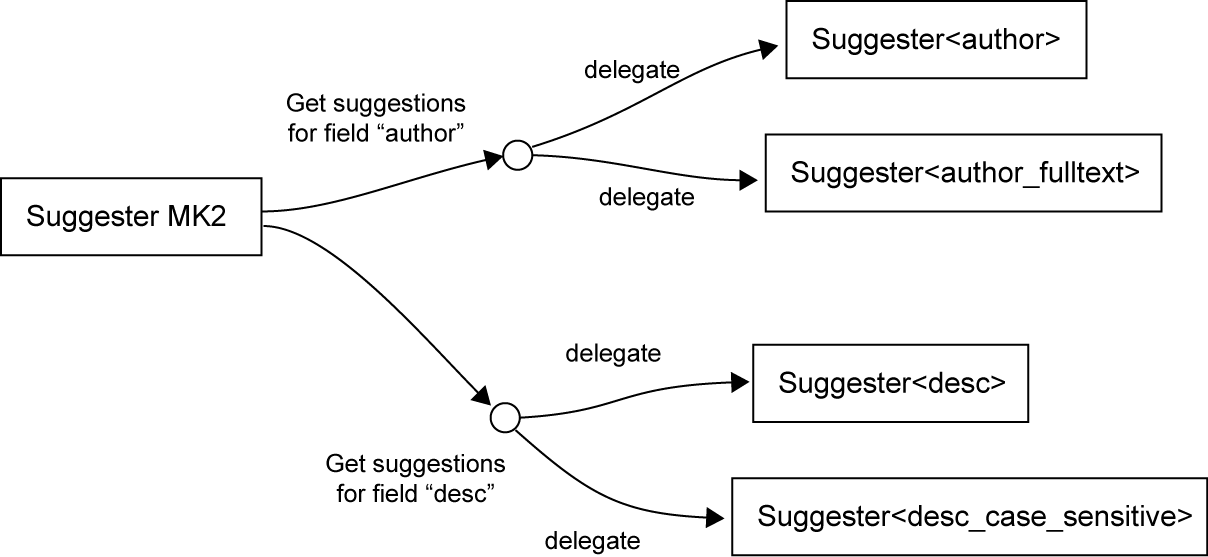
\includegraphics[width=0.8\textwidth]{img/delegation.png}
    \caption{Illustration of the delegation used by SuggesterMK2. The suggester will give suggestions drawn from the fields author and author\_fulltext for the field author, and from desc and desc\_case\_sensitive for the field desc.}
    \label{fig:delegation}
\end{figure}

Let us for instance say that we configure the system to give suggestions for the field |author| using the contents from the fields |author| and |author_exact|, the first of which being tokenized on whitespace, and the second being untokenized. All we have to do then, using delegation, is to construct a |Suggester| object for |author| and |author_exact|, query each of these, and then combine the results, merging results as needed if the results overlap. In our implementation, configuring the suggester to return results as in the diagram can be done by adding the following to the suggester configuration in |solrconfig.xml|:

\begin{verbatim}
<lst name="delegate">
  <str name="targetField">author</str>
  <str name="sourceField">author</str>
  <str name="sourceField">author_fulltext</str>
</lst>
\end{verbatim}

The fields we use for contents do not need to include the target field – we can use the contents from entirely different fields to use as suggestions. For a sample use case where this might be desired, consider what would happen if the target field were 4-gram tokenized: a word like ''parallelize'' would then be split up into the tokens ''para'', ''aral'', ''rall'', ''alle'', and so on, none of which we want to give as query suggestions. We would then want to draw suggestions from some other field where the contents are tokenized as words instead.

The |SuggesterMK2| implementation also gives query suggestions consisting of the field names it is configured to give suggestions for. For instance, the example configuration in figure \ref{fig:delegation} the |SuggesterMK2| would give |author:”| as a query suggestion when the user types |aut|.

For the full configuration of the suggester in solrconfig.xml, see Appendix.
For the implementation of the SuggesterMK2, see \cite{GITHUBPROJ}.

\subsubsection{Order of results}

The results of a query are returned in a given order. Field names are given priority over field contents, while field contents and standard results are both sorted based on number of occurrences. For example of this see section \ref{results}.

\subsubsection{Testing}

A simple frontend has been implemented to act as a tool for debugging and demoing the project. It uses JSON requests and responses to interact with the ''suggest'' and ''select'' features of the Solr server.

Testing was primarily done using the Solr Admin console and the frontend.
In the early stages of development, test data provided by Solr was used. This was replaced with a larger test set of documents containing fields for names, party affiliation and quotes from members of Swedish parliament later on. A number of queries were used to test that the suggester performed as expected. These queries, as well as the result of the tests for the final version, can be found in the following section. 


\section{Results}\label{results}

\section{Discussion}\label{discussion}

\subsection{Encountered issues}

Several issues were encountered while implementing the solution and these are described in the following sections. One should be careful to note the difference between query parameters, i.e. the parameters in the query passed to the indexing server, and document fields, i.e. fields in the documents indexed by the indexing server.

\subsubsection{Syntactical issues}

A number of symbols are considered special characters when they occur in a query. These include\cite{QUERY}:
\begin{verbatim}

+ - && || ! ( ) { } [ ] ^ " ~ * ? : \
\end{verbatim}

As a consequence of how the Solr request dispatch system is implemented, a query passed to Solr will be tokenized using the above characters as delimiters (except hyphen-minus), as well as on whitespace before being passed on to system modules like a suggester.
Consequently a sample query on the form: |author:"simon| will automatically be split into: |["author", "simon"]|
before being handed over to the suggester implementation.
Taking whitespace into account as well as a query on the form: |author:"simon AND text:"foo"| will automatically be split into the following: |["author", "simon", "AND", "text", "foo"]|.
Furthermore, while the order of the tokens seem to be preserved in practice, the documentation does not guarantee this.

The specifics of the tokenization can be changed in the Solr configuration by setting the |queryAnalyzerFieldType| in |solrconfig.xml|. Contrary to what is stated in the documentation though, Solr does not seem to actually respect the value of this field when tokenizing queries passed to the relevant component. This behaviour is present as of the currently penultimate version of Solr (version 4.7.2).

This particular issue can be circumvented by creating a custom parameter or by piggybacking on the Solr spellchecker implementation and using its custom |spellcheck.q| parameter instead (as the original query suggester implementation already does).
This parameter uses a tokenizer based on the type of the first defined parameter of name "field" in the definition of the component. |[http://mail-archives.apache.org/mod_mbox/lucene-solr-user/200906.mbox/%3C4A27D1FF.1070502@as-guides.com%3E]| 
Tokenization on special characters can be turned off simply by not defining any parameter called ‘’field’’ in the suggesters definition. This of course necessitates us to use some other way to specify which field to give query suggestions for, which is why we use the delegate syntax.

Using |spellcheck.q| removes tokenization on special characters, but still performs whitespace delimited tokenization. There does not appear to exist any simple way to avoid this phenomenon since it is already done by the point the suggester is given tokens. Also, the Lucene query parser for the original Solr query suggester does not respect phrase queries (i.e. not doing whitespace delimited tokenization when given queries surrounded by quotation marks). Thus while there might exist ways to avoid whitespace delimited tokenization, it does not appear possible with a drop-in replacement for the query suggester currently present in Solr.

To sum up, the least amount of tokenization that the drop-in replacement query suggester can get is: |author:"simon AND text:"foo"| being converted to: |["author:"simon", "AND", "text:"foo""]|, but, as already stated, the order of the tokens is not guaranteed to be preserved.

That whitespace delimited tokenization is unavoidable does not pose any obstacles to doing single word completion, of course, but it might make a multi word query completion implementation distinctly non-trivial. 

\subsubsection{Interpreting an unfinished query}

An unfinished query might be interpretable in multiple ways, for instance, the query: |author:"simon AND text:"foo| can either be interpreted as the intersection of two unfinished queries or as a search for the string ''simon AND text:'' in the field author and the string foo in any field. Another interpretation is to simply ignore the fact that the user has not closes the first field query and only supply suggestions for the string ''foo'' in the field text. 

When implementing multi-word query completion one might take the previous word into account when completing the next one. E.g. when completing the query: |author:"simon s| we might want to give priority to |author:"simon stenström"| over for instance |author:"simon simon"|.

This can in general be done using n-grams, but to our knowledge there are no tools in Solr for doing such tokenization\footnote{Note that the n-gram feature present in Solr is conceptually distinct from what we want here: it performs searches on letter n-grams which is useful for non-wordspaced languages like Chinese. What we require is word n-grams.}, and implementing this would be far outside the scope of this project. In the particular case, however, when for instance "Simon Stenström" is an actual value of the field "author" then one can do this kind of full field content completion quite simply by changing the type of the field "author" to some string based type that does not do whitespace tokenization (a better solution for the |SuggesterMK2| is to delegate to two fields that use different tokenization, which would yield both word and full text completion. Solr can be configured to copy field contents to other fields at indexing, by using so called copy fields, which means that the documents do not have to be alterated.).
However particular care must be exercised when considering what should happen when we attempt to query complete on a query on the form: |author:"simon s| as opposed to: |author:"sim| since the second query will readily be completed into either "simon" or "simon stenström" depending on the type of the field author, but the first will automatically be split into: |[author:"simon, s]| before we get our hands on it. We can of course disregard the second token and simply give suggestions on the first one, but then would also get completions like ''simon lundgren''.

In our implementation, we join the two tokens. This is based on the assumption that the order of the tokens has not been changed by the query parser, which as mentioned before seems to be the case in practice but is not guaranteed. 


\subsection{Need for configuration}

The way the design is made you need to configure the ||SuggesterMK2|| for each field that you want to provide query completion for. This gives great flexibility in what fields should be available for suggestions, which has many advantages. For example, you might want to limit access to some fields because they are not interesting from a user perspective. For some fields you might want to enforce tokenization on white space, if a field contains several rows of text you will want to return single words rather than the whole content.  Another advantage is the possibility to prevent query completion for fields that could contain sensitive information, thereby providing some security for the system.

Despite the advantages, special configuration for each field can seem a bit tedious. It is important to keep in mind though that Solr is often used for rather domain specific tasks, (e.g. Netflix or Instagram) and as such the number of fields that you’d want query completion for is also rather low. Therefore, the configuration is not really a problem.  

\subsection{Weighting between standard free text query completion and field query completion}

In this implementation, standard query completion (i.e. completion on actual content) is used in conjunction with field completion. If the |SuggesterMK2| is configured to provide suggestions for many fields, the field completion might overshadow the ordinary query completion results.
It is therefore of interest to consider if and how weighting should be done between standard and field completion. One way to counteract such behaviour would be to only match fields after a certain amount of characters have been entered, or when the match has reached a certain confidence level (e.g. edit distance).

In our implementation, suggestion for field names are always at the top. This is based on the fact that, as mention earlier,  Solr is rather domain-specific and therefore the likelihood of having so many fields that it causes problems is low.

\subsection{Unimplemented ideas}

In this section, a few unimplemented ideas are mentioned and difficulties with implementing these are discussed. 

\subsubsection{Intersection queries}

A good suggester iteratively builds a query, taking all previous text into account. This requires the suggester to construct queries along the way and then apply new filters to this original query as they are added. For example, for the query: |block:"Left" AND name:"p| we might only want to show name suggestions for left-wing members of parliament, otherwise we would actually suggest queries for which the search result would be empty.
However the original suggester implementation does not support intersection, and so we would have to manually remove inapplicable suggestion results (i.e. names of non-left-wing members of parliament in the above example) and adjusting the ranking of the results, as the ranking depends on the number of occurrences of the suggested words in the results. While this is most likely feasible, we consider this to fall well beyond the scope of this project.

\subsubsection{Query completion for AND and OR}

In Solr, the terms AND and OR can be used for intersection and union queries, respectively. 
A nice feature would be to support query completion for these terms so that when the user enters a whitespace after a query, the suggester gives suggestions for these terms, like the following example: |author:"simon" | which would be completed into: |author:"simon" AND|.

Since Solr automatically strips trailing and leading whitespace, this seems hard to do in the backend. One can easily do these kinds of query completions in the frontend however, and so we might question the need for having backend implementation for these in the first place.






\section{Conclusions}\label{conclusions}
blah blah blah...

\bibliographystyle{abbrv}
\bibliography{references}

\newpage
\section*{Appendix}\label{appendix}

\subsection*{Sample queries}
\begin{tabular}{ r | l}
    Query & Completion suggestions \\    
    \hline                    
    & \\
  |n| & |name:"| \\
      & |nilsson| \\
      & |näringsminister| \\
      & |näringsminister annie lööf| \\
      & |nina larsson| \\
      & |nina lundström| \\
      & |nylander| \\
      & |nylund| \\
      & \\
    \hline
    & \\
  |name:"d| & |name:"désirée| \\
            & |name:"david lång| \\
            & |name:"douglas| \footnotesize{(note: surname)}\\
            & |name:"désirée liljevall| \\
            & |name:"désirée pethrus| \\
            & \\
    \hline
    & \\
    |name:"désirée p| & |name:"désirée pethrus| \\
    & \\
    \hline
    & \\
    |name:"foo" AND name:"d| & |name:"foo" AND name:"désirée| \\
                           & |name:"foo" AND name:"david lång| \\
                           & |name:"foo" AND name:"douglas| \\
                           & |name:"foo" AND name:"désirée liljevall| \\
                           & |name:"foo" AND name:"désirée pethrus| \\
                           & \\
    \hline
    |name:"foo" AND name:"désirée p| & |name:"foo" AND name:"désirée pethrus| \\
\end{tabular}

\begin{tabular}{ r | l}
|name:"nina AND p| & (No results since there are no words in the data \\ & beginning with the exact phrase |nina AND p|) \\
\hline
|name:"nina" AND p| & |name:"nina" AND party:"| \\
                    & |name:"nina" AND patrik björck| \\
                    & |name:"nina" AND peter eriksson| \\
                    & |name:"nina" AND peter persson| \\
                    & |name:"nina" AND pia hallström| \\
                    & |name:"nina" AND pia nilsson| \\
                    & |name:"nina" AND polfjärd| \\
                    & |name:"nina" AND pyry| \\
                    &  \hspace{66pt} \vdots 
\end{tabular}


\newpage

\subsection*{solrconfig.xml additions}

\begin{verbatim}
  <!-- ir14 -->
    <searchComponent class="solr.SpellCheckComponent" name="suggest">
    <lst name="spellchecker">
    <str name="name">suggest</str>
    <str name="classname">org.DD2476.SuggesterMK2</str>
    <str name="lookupImpl">org.apache.solr.spelling.suggest.tst.TSTLookupFactory</str>

        <!--
        Define delimiters to use for splitting queries into
        field name/field values. If several are specified, it will
        return results using the same delimiter as in the query.
        If no delimiter is used in the query, but a delimiter is to
        be returned, the first delimiter specified below is used.
        If no delimiter is specified, :" is used.
    -->
    <str name="delimiter">:"</str>
    <str name="endDelimiter">"</str>

    <!--
    Define suggesters for the fields you want to enable auto
    completion for. Requires a target field, ie. the name of the
    field that is sent in the query. If a source field is
    specified, it will be used to fetch suggestions from.
    If left unspecified, the target field will be used.
    Several source fields can be specified.
    If no delegate is specified at all, every field will be used
    as target field and source field respectively.

    Example:

    <lst name="delegate">
        <str name="targetField">author</str>
        <str name="sourceField">author</str>
        <str name="sourceField">author_ir14_auto_complete</str>
    </lst>

    The above will allow the user to get query completion for the 
    field author and will fetch suggestions from the fields     author and author_ir14_aut_complete.
    -->
    <lst name="delegate">
          <str name="targetField">name</str>
          <str name="sourceField">name</str>
          <str name="sourceField">name_ir14_auto_complete</str>
    </lst>

    <lst name="delegate">
          <str name="targetField">party</str>
          <str name="sourceField">party</str>
    </lst>

    <lst name="delegate">
          <str name="targetField">birthyear</str>
          <str name="sourceField">birthyear</str>
    </lst>

     <lst name="delegate">
          <str name="targetField">block</str>
          <str name="sourceField">block</str>
     </lst>
     
    <float name="threshold">0.005</float>
    <str name="buildOnCommit">true</str>
    </lst>
  </searchComponent>
\end{verbatim}




\end{document}